\documentclass[../main.tex]{subfiles}

\begin{document}

\section{Overview}

This chapter presents the goals and ongoing development of the LeafAI web application, an interactive user-facing application which integrates with the LeafAI API described in Chapter \ref{chap:query_generation}. As we determined evaluation of the web application to be out of scope for the current project, we leave this to future work.

\section{Related Work}

Experimental systems enabling the querying of databases using natural language interfaces have been in development since the 1960s. Using relatively simple rule-based parsing systems, Woods \cite{woods1973progress} created a system for asking natural language questions of a moon rock database, while Epstein and Walker \cite{epstein1978natural} similarly designed a natural language interface for a melanoma database. Decades later, Katz \textit{et al} created START \cite{katz1999integrating}, a system capable of basic question-answering using data extracted and parsed from the internet. In the biomedical informatics domain, Cao \textit{et al} developed AskHERMES \cite{cao2011askhermes}, question-answering software capable of answering medical questions related to drugs, contraindications, and so on, using support vector machines (SVMs) and an internal knowledge base derived from the UMLS.

Cohort discovery systems using natural language are in many ways a subset of systems for question-answering which answer only one unstated question, "How many patients meet these criteria?". In the biomedical informatics and clinical trials domain, the most well-known and cited system for matching patients to clinical trials using free-text eligibility criteria is Criteria2Query \cite{yuan2019criteria2query, fang2022combining}. Criteria2Query offers a web-based simple and friendly user interface for inputting free-text eligibility criteria. The system analyzes user inputs and returns a highlighted listing of named entities it identified, as well as a potential list of patients meeting those criteria from an OMOP database.

\section{Methods}

LeafAI will be developed using a 3-tier architecture similar to Leaf \cite{dobbins2019leaf}: a back-end with clinical and application databases, and server hosting an API (discussed in Aim 2), and a front-end web application. The key innovation of the web application will be its user interface, a chat-like design we expect will be familiar to most users of applications such as Microsoft Teams or Slack.

A chat-like interface for cohort discovery is both novel and a logical design choice given the natural language interface of LeafAI used for query generation. An example of LeafAI's proposed chat interface is shown in Figure \ref{fig_leafai_demo}. As can be seen, we assume that the order of user-provided criteria is intentional and important, and leverage that assumption to both structure queries incrementally to report results line by line, with each reported result (e.g., "421 are aged between 18 and 65") effectively a subset of the preceding result.

\begin{figure}[h!]
  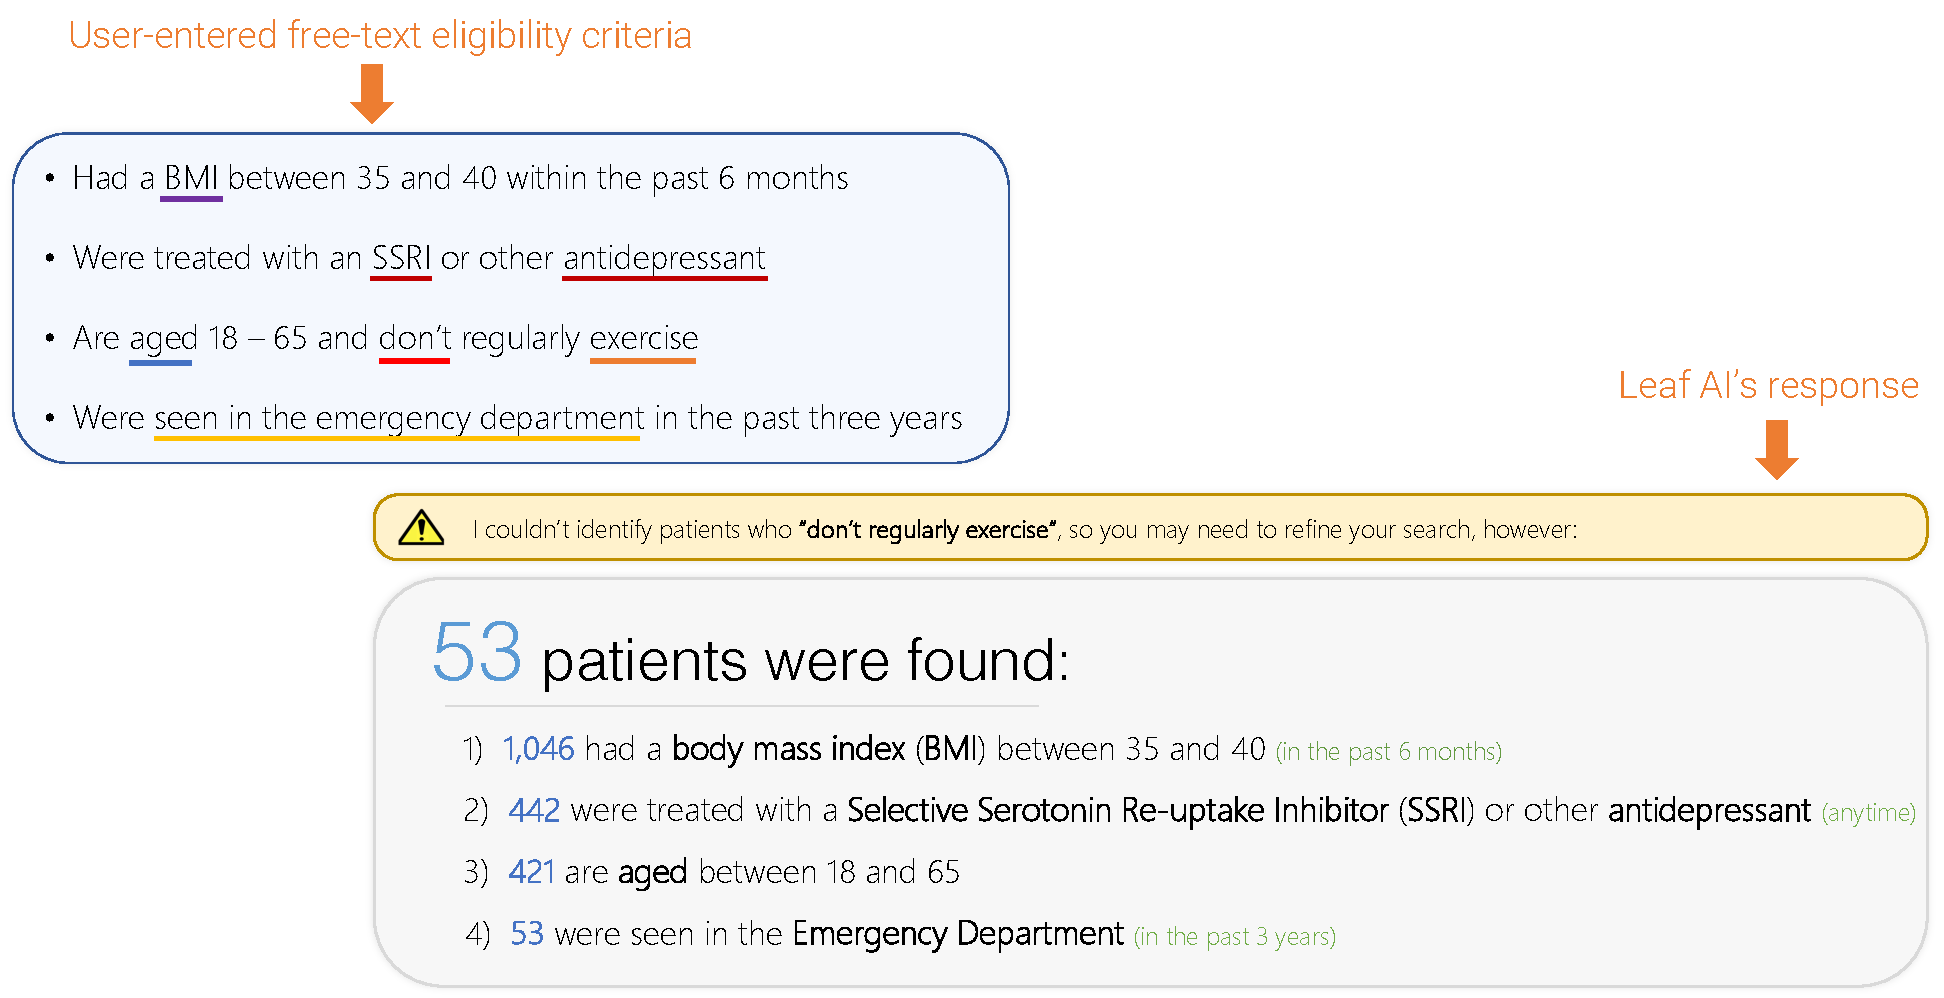
\includegraphics[scale=0.58]{Figures/8_web_application/leafai_demo.pdf}  
  \caption{A example mockup of the LeafAI user interface. User-entered criteria are shown in the above left, while LeafAI responses are shown in the lower-right. User criteria are displayed and executed in order, with each count of patients representing a subset of the preceding count.}
\label{fig_leafai_demo}
\end{figure}

It is important to emphasize that LeafAI will respond using a visual form that is chat-\textit{like}, rather than itself being a chat\textit{bot} (i.e., a programmatic conversation agent). While the user interface and query generation methods described in Aim 2 lay a potential foundation for general-purpose question-answering more akin to a conversation agent, we leave that to future work and limit our scope in this project to cohort discovery. The user interface of LeafAI will have the following goals:

\begin{enumerate}
    \item \textbf{Accessible history}. Users will be able to immediately scroll to view previous findings.
    \item \textbf{Rapid feedback and explainability}. LeafAI while perform NER and normalization as users are typing, similar to prefetching search engine responses. This will allow users to preemptively detect concepts and queries which may return unexpected results. LeafAI will also display incremental query results in real-time, providing users faster feedback so users may avoid waiting until all query results are complete.
    \item \textbf{Direct editing of responses enabling iteration}. As LeafAI returns results of patients found, the eligibility criteria used in a query will be directly edit-able, saving users' time and facilitating quick iteration to find intended patients.
\end{enumerate}

\noindent We next describe each goal in detail.

\subsection{Accessible History} 

Cohort discovery is a form of data exploration. As Derthick and Roth write, "...the data exploration process is not characterized by monotonic progress towards a goal, but rather involves much backtracking and opportunistic goal revision" \cite{derthick2001enhancing}. Put another way, user goals and perceptions may change over the course of their exploration. With ubiquitous vertical scrolling - where more recent actions and utterances are inserted downward while history is preserved upward - chat-like user interfaces facilitate user understanding of past utterances and actions. Persisted, easily viewable history of user utterances and actions enable what Gergle \textit{et al} call "conversational grounding" \cite{gergle2004persistence}, that is, accessible data to guide users to previously acquired findings and information. This history of previous actions can improve the pace of discovery and alleviate the need for users to (often imperfectly) attempt to recall their earlier findings and paths taken \cite{hill1994history, gergle2004persistence}.

\subsection{Rapid Feedback and explainability}

Users' sense of system latency and responsiveness can significantly affect their satisfaction in using a tool \cite{li2019effects, arapakis2014impact, shneiderman1984response}. Faster \textit{preemptive} system responses (i.e., informing users' of a possible consequence before they complete an action) can also both save users' time and reduce loads placed upon systems by preventing unnecessary actions \cite{lempel2003predictive, diaz2016search}. LeafAI will employ two general strategies for providing rapid feedback to users, one before queries are executed, and the second while results are being reported during query execution.

First, consider a hypothetical case where a user begins to type a criteria but misspells "Diabetes Mellitus". The user may take seconds or even minutes of additional typing while adding new criteria without knowing of the initial spelling mistake. After the user awaits LeafAI's response, she finds that the query found no patients and is frustrated and confused at the counter-intuitive result, only to finally notice the misspelling, having wasted several minutes. We aim to avoid this scenario by preemptively performing NER and normalization while users are typing. Examples of this are shown in Figure \ref{fig_leafai_mouse_hover}. Named entities found within user criteria will be underlined and interactive, enabling users to better estimate whether their queries will succeed or not.

\begin{figure}[h!]
  \centering
  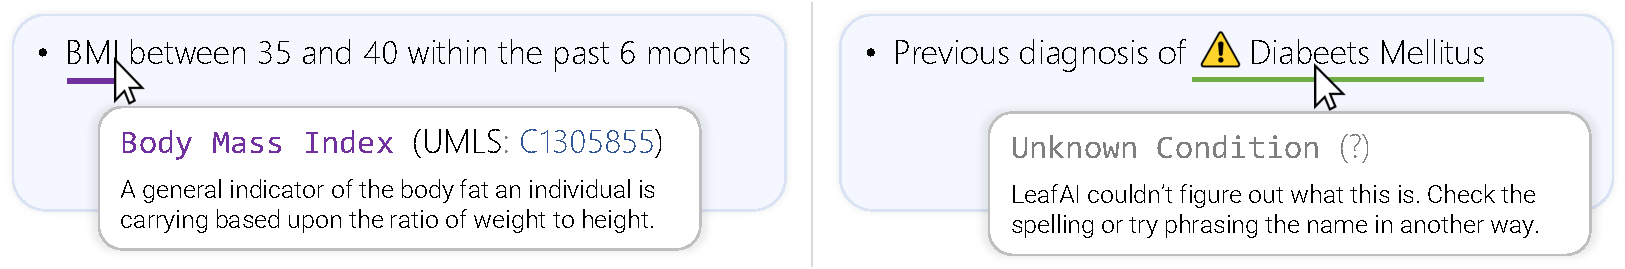
\includegraphics[scale=0.68]{Figures/8_web_application/leafai_mouse_hover.pdf}  
  \caption{Normalized named entities identified in user input before query execution. On the left, the system correctly identified "BMI". On the right, "Diabetes Mellitus" is misspelled, and the user is notified.}
\label{fig_leafai_mouse_hover}
\end{figure}

Second, as LeafAI generates incremental queries and returns results line by line asynchronously, the user interface will show results as they are reported using a streaming interface. As a result, users will not need to wait until all queries are complete (as in tools such as Leaf and i2b2). An example of this is shown in Figure \ref{fig_leafai_query_progress}.

\begin{figure}[h!]
  \centering
  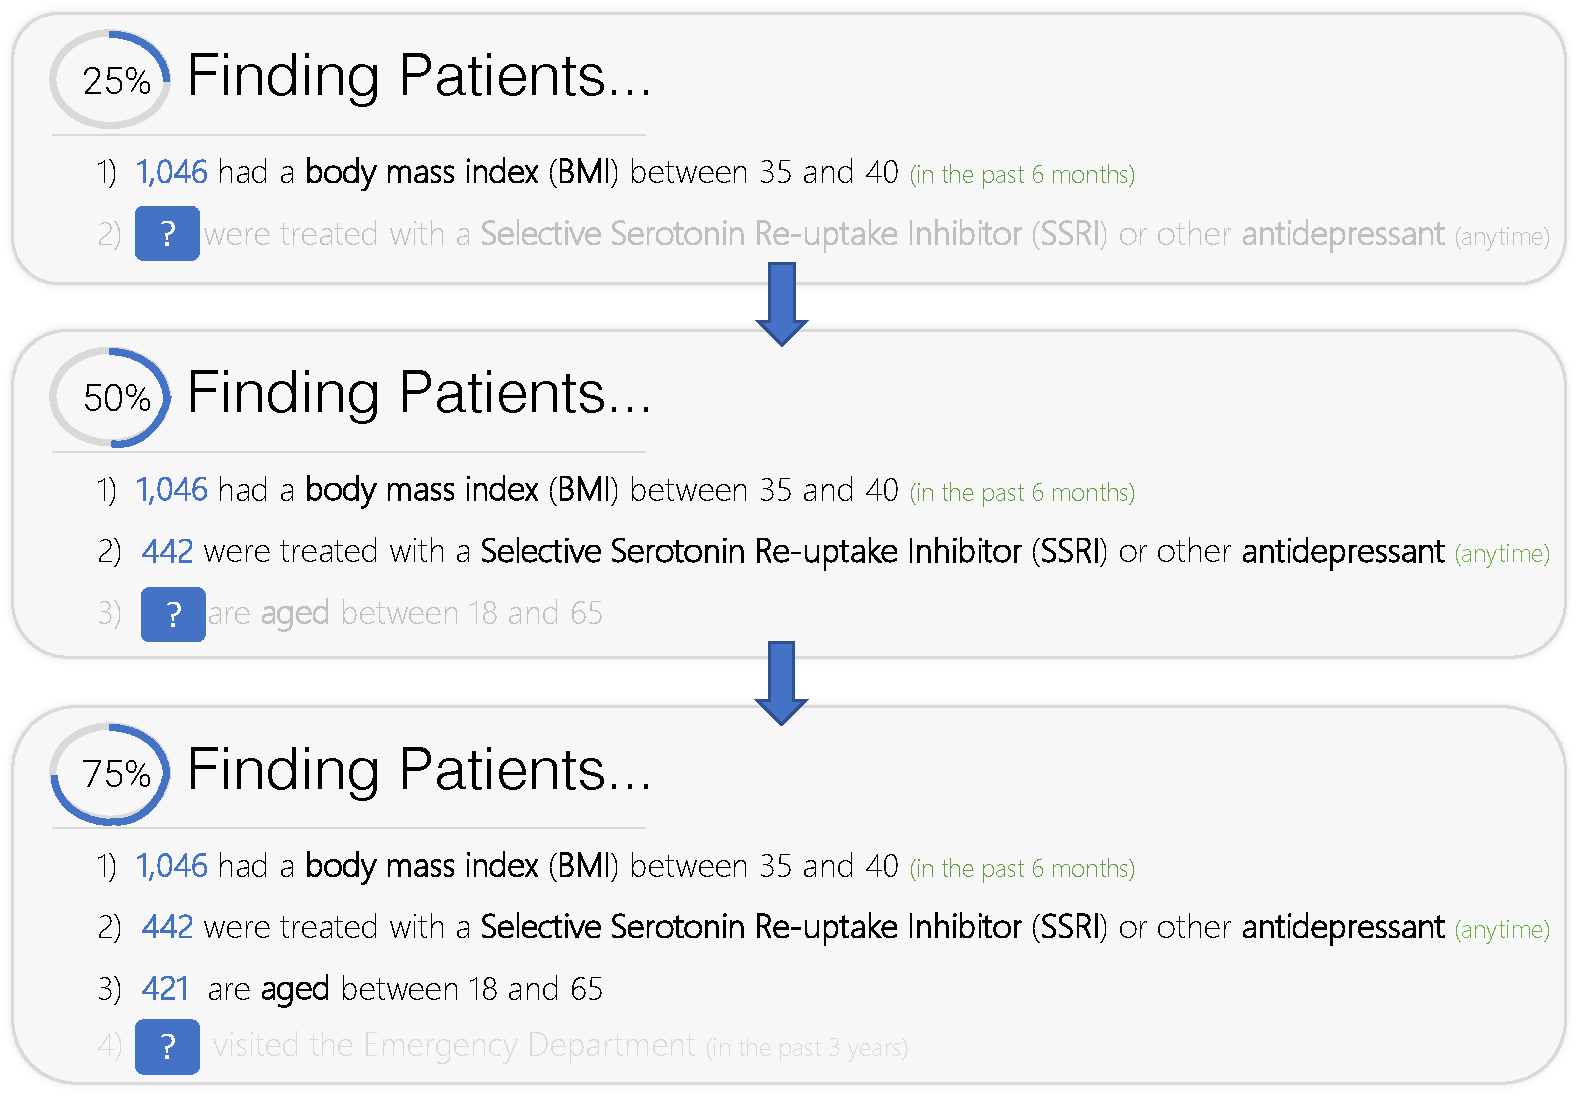
\includegraphics[scale=0.5]{Figures/8_web_application/leafai_query_progress.pdf}  
  \caption{A time-lapse style representation of the user interface asynchronously reporting incremental query results, from top to bottom. This will be performed using two streaming interfaces, one from the clinical database to the API, and a second from the API to the web application.}
\label{fig_leafai_query_progress}
\end{figure}

Taken together, these features for rapid feedback and transparency also enable \textit{explainability} of system actions. That is, rather than simply returning a final count of patients meeting criteria, LeafAI will provide information both before and during query execution of how the system interpreted user intent and how it has executed a query (e.g. what concepts it found or did not, misinterpreted, etc.). We currently plan for system language for explaining query results to be generated by templated English expressions mapped to logical form types "slot-filled" using normalized UMLS concept names. By avoiding being a "black box", we expect these features to help gain user trust and understanding of both the system's successes and shortcomings.

\subsection{Direct editing of responses enabling iteration}

Data exploration is iterative: users explore, try, and learn over the course of multiple attempts. As discussed, faster, meaningful results also directly affect user satisfaction. To this end, LeafAI will allow users to immediately and directly edit the responses returned by LeafAI. This workflow is depicted in Figure \ref{fig_leafai_feedback_loop}. 

\begin{figure}[h!]
  \centering
  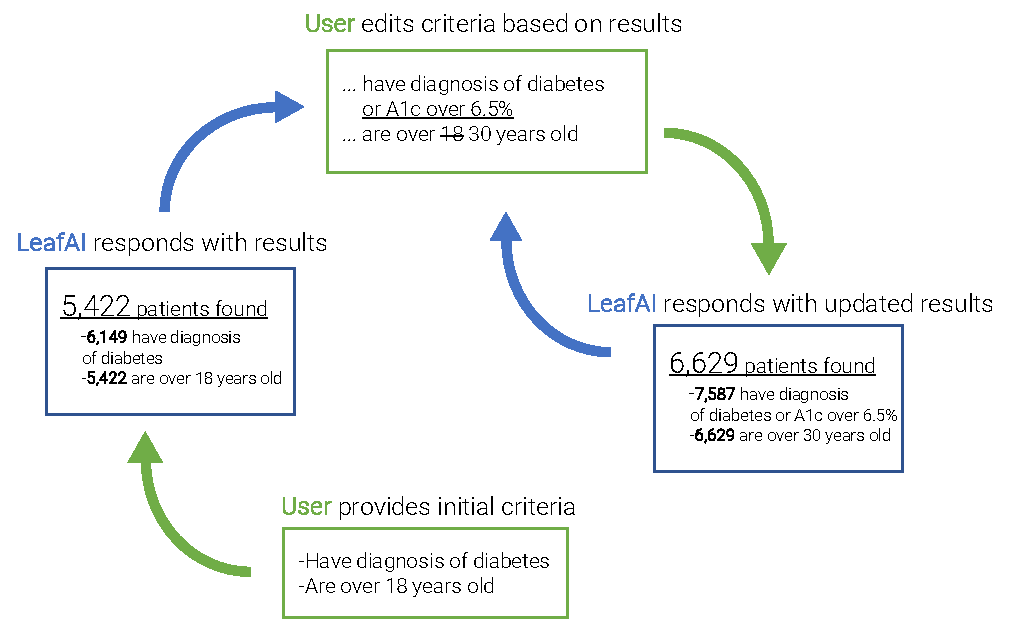
\includegraphics[scale=1]{Figures/8_web_application/leafai_feedback_loop.pdf}  
  \caption{An iterative workflow using an example case for adults with Diabetes Mellitus. Users will be able to directly edit results and re-execute their queries while preserving query history, saving user time and preserving previous user actions and findings.}
\label{fig_leafai_feedback_loop}
\end{figure}

For example, after seeing that LeafAI found less patients than expected, a user may realize that she should slightly alter her original query to expand her search. Rather than needing to copy and paste her earlier criteria, instead she will be able to simply click and modify the earlier results.

Additionally, LeafAI is capable of reasoning upon non-specific criteria. In certain cases, however, the system's findings may be incomplete, incorrect, or undesired for various reasons. Rather than forcing users to accept imperfect reasoning, however, LeafAI will allow users to directly edit reasoned concepts. An example of this is shown in Figure \ref{fig_leafai_edit}.

\begin{figure}[h!]
  \centering
  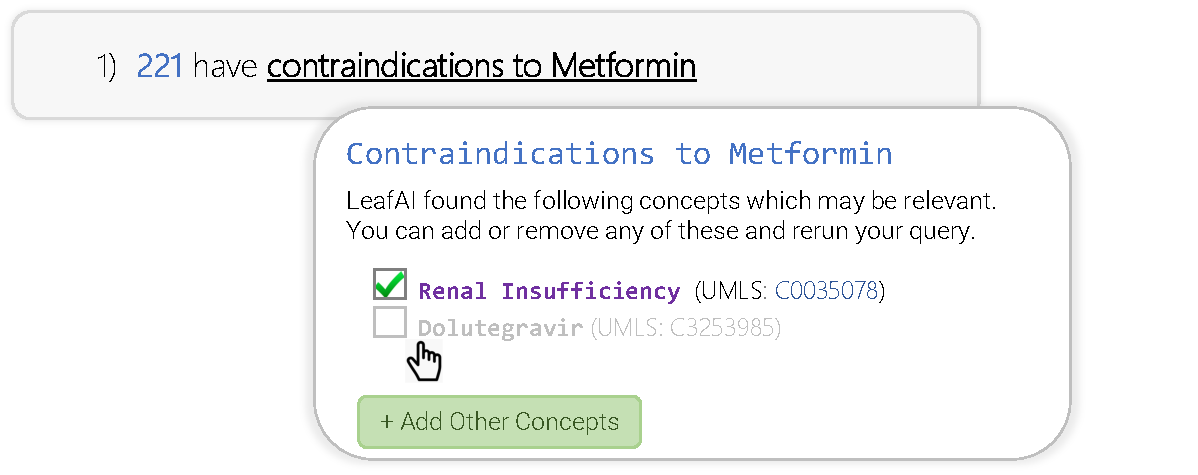
\includegraphics[scale=0.68]{Figures/8_web_application/leafai_edit.pdf}  
  \caption{An example of a user editing concepts discovered using LeafAI's reasoning system. Users will be able to add or remove reasoned concepts.}
\label{fig_leafai_edit}
\end{figure}

The system's reasoning can thus be described as an optional means of helpfully saving users' time, which can be accepted, edited, or discarded as needed.

\subsection{Model Inference Speed}

LeafAI's modules for NER, logical form transformation, lab normalization and so on use large Transformer-based neural models \cite{vaswani2017attention} with millions of parameters. Using these models as-is for inference can be slow, particularly when performed using CPUs rather than more costly but often far faster GPUs (Graphics Processing Units). Delays in inference time in turn can result in poor system latency, affecting user satisfaction. We further assume that institutions or individuals deploying LeafAI may not necessarily have access to GPUs. To improve inference speed on CPUs, we intend to quantize our models, a process for converting 32-bit floating point values within model weights and biases to 8-bit integers. Quantization has been shown to dramatically reduce model storage size and memory usage and improve inference speed while typically showing limited decreases in performance \cite{hubara2017quantized}. 

\section{Conclusion}

\end{document}